%----------------------------------------------------------------------------------------
%	PACKAGES AND THEMES
%----------------------------------------------------------------------------------------
\documentclass{beamer}
\usetheme[nomail, nogauge, delaunay, amurmapleblack]{Amurmaple}
\usepackage[french]{babel}
\usepackage{hyperref}
\usepackage{graphicx} % Allows including images
\usepackage{booktabs} % Allows the use of \toprule, \midrule and \bottomrule in tables
\usepackage{animate}
\usepackage{tikz}
\usepackage{graphicx}
%----------------------------------------------------------------------------------------
%	TITLE PAGE
%----------------------------------------------------------------------------------------

% The title
\title[Présentation de l'association]{Présentation de l'association Centrale Mathématiques}

\author[Centrale Mathématiques] {Mathis Rimbert, Maxime Haberthur, Raphaël Casanova}
\institute[NTU] % Your institution may be shorthand to save space
{
}
\date{\today} % Date, can be changed to a custom date


%----------------------------------------------------------------------------------------
%	PRESENTATION SLIDES
%----------------------------------------------------------------------------------------

\begin{document}

\begin{frame}
    % Print the title page as the first slide
    \titlepage
\end{frame}

\sepframe[title = {Sommaire}]



%------------------------------------------------
\section{Présentation générale}
%------------------------------------------------

\begin{frame}{Présentation}
  \framesection{Raison d'existence de l'association :}
  \begin{itemize}
    \item Beaucoup d'options de cursus liés aux maths à Centrale (licence, électifs, DD)...
    \item ...Mais aucune structure pour promouvoir la culture mathématiques
  \end{itemize}
  On constate donc que pour ceux qui apprécient les mathématiques (et la science en général), il est impossible de s'engager associativement dans ce domaine.

  \framesection{Objectifs de l'association :}
  \begin{enumerate}
    \item Promouvoir la culture mathématiques à l'Ecole Centrale de Lille
    \item Fournir un espace de travail et du support aux étudiants
  \end{enumerate}
\end{frame}

\begin{frame}{Organigramme du Bureau}
  \begin{tikzpicture}

    % Création d'un chemin pour bien espacer les noeuds
    \path (0,0) node (president) [draw, rectangle, minimum width=2cm, minimum height=2cm] {
        \begin{tabular}{c}
            
\includegraphics[width=1.65cm]{./images/rimbert.png} \\
            \textbf{Mathis Rimbert} \\
            Président
        \end{tabular}
    }
    \path (3.9,0) node (secretaire) [draw, rectangle, minimum width=2cm, minimum height=2cm] {
        \begin{tabular}{c}
            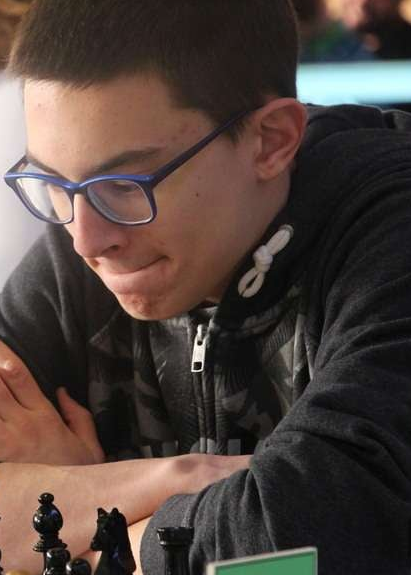
\includegraphics[width=1.79cm]{./images/haberthur.png} \\
            \textbf{Maxime Haberthur} \\
            Secrétaire
        \end{tabular}
    }
    \path (8,0) node (tresorier) [draw, rectangle, minimum width=2cm, minimum height=2cm] {
        \begin{tabular}{c}
            
\includegraphics[width=2.5cm]{./images/casanova.png} \\
            \textbf{Raphaël Casanova} \\
            Trésorier
        \end{tabular}
    };
    
    \end{tikzpicture}
  \end{frame}
  

%------------------------------------------------
\section{Services et utilité}
%------------------------------------------------
\begin{frame}{Services et utilité}  
  \framesection{Organisation de conférences mathématiques}
  \begin{itemize}
    \item Proposer à des chercheurs ou à des doctorants de venir présenter leurs travaux
    \item Proposer des mini-cours sur des sujets pouvant intéresser les Centraliens
  \end{itemize}

  \framesection{Formation à l'outil \LaTeX}
  \begin{itemize}
    \item Réaliser une présentation (comme celle-ci) en \LaTeX, un CV, une lettre, un document scientifique etc.
  \end{itemize}

  \framesection{Aide en mathématiques}
  \begin{itemize}
    \item Revoir quelques exercices avant les partiels d'AIN ou de MAC (ou de mathématiques pour les ITEEMiens)
    \item Proposer des corrigés des partiels et des exercices pour la licence conventionnée avec Centrale
  \end{itemize}

\end{frame}

%------------------------------------------------
\section{Besoins}
%------------------------------------------------
\begin{frame}{Besoins de l'association}
  Nous avons pu, lors de nos discussions, voir émerger plusieurs besoins pour le bon fonctionnement de l'association :
  \begin{itemize}
    \item Avoir un lieu pour se réunir, échanger, écrire sur un tableau, stocker des documents (livres, compte-rendu papier des conférences...) nous semble être primordial. 
    \item Obtenir éventuellement un budget modéré pour financer l'achat de ressources mathématiques ou éventuellement défrayer les intervenants pourrait permettre à l'association de croître plus rapidement.
  \end{itemize}
\end{frame}

  
\thanksframe{Merci de votre attention !}





\end{document}